\def\checkmark{\tikz\fill[scale=0.4](0,.35) -- (.25,0) -- (1,.7) -- (.25,.15) -- cycle;}

\begin{abstract}Examination is one of the few parts of education which has not profited from digitalization. However, electronic examination can make the assessment process faster and more valid. Especially, with respect to the current pandemic, e-exams are not only an opportunity for improvement but have become necessary. To ensure sound e-assessments, an examination system must meet certain requirements. We develop these requirements and give insight into the design principles that help us match them. These design principles are used to evaluate popular e-examination tools. We find none of them fully meeting the proposed requirements. Especially, in areas of cheating prevention and protection against contestation these tools fall short. With the aim of constructing a better solution, we propose an examination tool prototype. In order address the shortcomings of the other tools, this prototype provides offline capabilities and per question time constraints. It thus lays a foundation for modernizing exams.\end{abstract}
\newpage
\newglossaryentry{sample}{name={sample},description={an example}}
\printglossaries
\newpage
\tableofcontents

\newpage

\hypertarget{introduction}{%
\section{Introduction}\label{introduction}}

\gls{sample} is Examinations make up a crucial part of education. Great
amounts of time go into organizational overhead. Although digitalization
has found its way into many parts of education, assessment largely is
not one of them. However, a step towards digital examination (e-exams)
would make the assessment process more flexible, scalable and
resource-efficient. Meanwhile, e-exams can lead to a more accurate
depiction of a students' competence.

In general, e-exams are advantageous in numerous ways. Their digital
nature makes exam data easy to analyze. This analyzing creates insights
into the performance of students and the quality of exam questions.
Compared to paper based exams, logistics become more efficient, as
physical answer sheets must no longer be moved around. As an exam is no
longer bound to the physical answer sheet, exam are no longer
location-bound. Exams could be taken at any place with internet and
power connection. This reduces efforts in exam location planning.
Additionally, archiving exams becomes faster and more space-efficient.
Further, we find advantages in the way questions are asked. Question
formats are no longer bound to paper. Thus, more application-oriented
questions can be asked and knowledge can better be assessed.

Digitizing exams is no novel idea. However, many concepts and
implementations focus on conducting e-exams in the same physical
environment as \emph{paper-based exams} (Vogt and Schneider
\protect\hyperlink{ref-Vogt2009}{2009}). This results in exams that are
either conducted on the universities' hardware (Johannes
Gutenberg-Universität Mainz
\protect\hyperlink{ref-JohannesGutenberg-UniversitatMainz}{2018}) or in
so-called \emph{bring-your-own-device} (\emph{BYOD}) exams (Peregoodoff
\protect\hyperlink{ref-GLM2015}{2015}). The former is associated with
high investments in computer infrastructure. It is evident, that
students need to own an electronic device (e.g., a tablet or laptop) to
participate in university. Taking this into consideration, \emph{BYOD}
solutions become the most sensible option.

In the face of a global pandemic, the gathering of large groups of
students poses health risks. The organization of exam locations, thus,
has become increasingly more difficult. More locations with larger areas
are needed in order to fulfil the needs of assessments. As discussed
above, using the examinees' own device, e-exams can be taken
independently of any location planning--even at the examinees' own home.
This decentralization eliminates the overhead that results from the
allocation of locations to different exams.

Taking these points into consideration, we will discuss decentralized
e-exams in more depth. It is important to notice, that
\emph{decentralized e-exams} differ from \emph{paper-based exams} and
\emph{centralized e-exams} in several key points. Foremost, the examiner
has less control over the environment under which the exam is taken.
This raises questions about exam integrity and fairness. These questions
must be addressed through careful conceptualization of questions and
careful software design.

Evidently, to some degree \emph{e-exams} are already conducted today.
Some solutions, for example, make use of a \emph{proctoring system}. In
such a system, a supervisor can access the examinees' device, he can
monitor all the students activities and surveil them through their
webcam. Proctoring of students aims to prevent or at least detect
cheating. However, this approach is costly, it hardly scales and
provides no real protection against cheating. Furthermore, test-taking
applications are found in many \emph{Learn Management Systems (LMS)}.
These systems are especially well suited for self-assessment. Their
suitability for a real exam majorly varies in quality.

This thesis thus focuses on decentralized e-exams that renounce the
usage of a proctor. For this purpose, we identify requirements that need
to be met to allow for a sound exam. We then find design principles that
help us match these requirements. As a guideline, this thesis uses a
design-oriented research approach. Hevner et al.
(\protect\hyperlink{ref-Hevner2004}{2004}) propose guidelines to conduct
design-oriented research. This thesis pursues these guidelines as
follows:

\begin{enumerate}
\def\labelenumi{\arabic{enumi}.}
\tightlist
\item
  \textbf{Design as an artifact:} The result of this research project is
  an IT artifact. It provides an implementation of a specific electronic
  exam. This artifact acts as a prototype for a product that ultimately
  aims to be used in the real-world examination process.
\item
  \textbf{Problem relevance:} Exams are the only part of education that
  has not made use of digitalization. E-exams could allow for a cheaper
  and more accurate way of assessing students.
\item
  \textbf{Design evaluation:} The effectiveness of the artifact is based
  on the effectiveness of design principles that are derived from
  research and intuition.
\item
  \textbf{Research contribution:} There are few systems designed for
  providing high validity. Many systems that do exist, make use of
  \emph{proctoring environments} (the student is continuously
  surveilled) which are expensive and can still be fooled. This research
  artifact aims to minimize academic dishonesty through design
  decisions.
\item
  \textbf{Research rigor:} This thesis builds upon research in the
  fields of education. It takes into account what other universities
  have already incorporated into their examination process and what
  empirical studies have shown to be valuable and efficient.
\item
  \textbf{Design as a search process:} Digital exams are no new concept.
  Still, it is not widely adopted. This thesis builds upon the works of
  different software artifacts and research conducted in the field of
  education.
\item
  \textbf{Research communication:} This thesis focuses on illustrating
  design considerations that were made in order to develop an artifact
  that most closely fits the needs of sound assessment. Therefore, this
  thesis focuses more on the concept and design principles needed to
  achieve a suited examination system. However, as we developed a
  prototype for conducting exams, we will also cover the technical
  implementation of various design principles.
\end{enumerate}

\newpage

\hypertarget{requirements-for-e-exams}{%
\section{Requirements for E-Exams}\label{requirements-for-e-exams}}

We find e-exams to be advantageous in a variety of ways. Still, it must
be ensured that e-exams meet the same standards that are asked for in
paper-based exams. For this cause, we define requirements as a framework
for any examination. Handke and Schäfer
(\protect\hyperlink{ref-Handke2012}{2012}) provide such requirements. In
this thesis, we ask how to design sound e-examination software. For this
purpose, we focus on topics that are directly influenced by such
software. We do not consider issues concerning the content of the exam.
Further, we divide the given requirements into three broad categories:

The first requirement defines the desired outcome of an exam:

\begin{enumerate}
\def\labelenumi{\arabic{enumi}.}
\tightlist
\item
  \textbf{General Validity.} Exams should aim to provide an accurate
  depiction of an examinees' competence level.
\end{enumerate}

Further, we find requirements that mainly influence interactions of
examinees and examiners with the examination system:

\begin{enumerate}
\def\labelenumi{\arabic{enumi}.}
\setcounter{enumi}{1}
\tightlist
\item
  \textbf{Protection against contestation.} No formal or technical
  deficiencies should occur that question the validity of the exam.
\item
  \textbf{Equal treatment.} Individual examinees must be treated
  equally.
\item
  \textbf{Protection against cheating.} The exam's outcome must be
  protected against manipulation by examinees.
\item
  \textbf{Transparency.} The examination process and results must be
  understandable and verifiable.
\end{enumerate}

Lastly, we determine requirements that mainly influence the technical
implementation of how the examination system handles data:

\begin{enumerate}
\def\labelenumi{\arabic{enumi}.}
\setcounter{enumi}{5}
\tightlist
\item
  \textbf{Protection of data.} The data of examinees is personal. As
  such it must be protected from misuse.
\item
  \textbf{Integrity.} Exam data must maintain consistency, accuracy and
  trustworthiness throughout its entire lifetime.
\item
  \textbf{Attributability.} A taken exam must uniquely map to a single
  examinee and vice versa.
\end{enumerate}

These categories set a general framework of how to design any
examination system. Table \emph{1} shows the design principles needed in
order to match the requirements mentioned above. In the following, we
will discuss these design principles.

\begin{center}
\def\arraystretch{1.5}
\begin{table}
\begin{tabular}{ | l | p{9cm} |}
\hline
Requirement & Design Principle \\ \hline

\multirow{2}{6cm}{1. General Validity}

& \textbullet Per question time constraints \\
& \textbullet Multiple question types \\ \hline

\multirow{2}{6cm}{2. Protection against contestation}

& \textbullet Offline capabilities \\
& \textbullet Students should be advised to ensure a reliable exam environment \\ \hline

\multirow{2}{6cm}{3. Equal Treatment}

& \textbullet Device agnostic \\
& \textbullet Exams must leverage automation wherever possible \\ \hline

\multirow{4}{6cm}{4. Protection Against Cheating}

& \textbullet Creation and management of large question pools \\
& \textbullet Per question time constraints \\
& \textbullet Randomization of question order \\
& \textbullet Providing a sense of surveillance \\ \hline

\multirow{2}{6cm}{5. Transparency}

& \textbullet Examiners must be able to give feedback to answers \\
& \textbullet Feedback must be reviewable by students \\ \hline

\multirow{3}{6cm}{6. Protection of Data, 7. Integrity and 8. Attributability }

& \textbullet User rights management \\
& \textbullet User action logging \\
& \textbullet Codebase is open source \\ \hline

\end{tabular}
\caption{\label{tab:Requirements_with_matching_design_principles}Requirements and their respective design principles}
\end{table}
\end{center}

\hypertarget{general-validity}{%
\subsection{General Validity}\label{general-validity}}

Examinations should support the purpose of universities to produce
highly capable individuals (Halbherr et al.
\protect\hyperlink{ref-Halbherr2014}{2014}). The measurement of success
in that aspect is largely based on the students' performance in exams.
Subsequently, students are highly incentivized to focus their studies on
a specific exam format and its question types. This interdependency
between knowledge acquisition and the examination shows the importance
of exam design. Further, it poses the question of what and how to test.
We find different question types to be particularly well suited for
testing specific aspects of learning. These question types can be
defined as follows (Halbherr et al.
\protect\hyperlink{ref-Halbherr2014}{2014}):

\begin{itemize}
\tightlist
\item
  \textbf{(Semi) Closed questions}, mainly revolve around the
  demonstration of \emph{factual knowledge}. Solutions are not
  disputable; there are only right and wrong answers. Typical answer
  formats include multiple-choice and simple text . \emph{For example:
  ``What does \emph{BYOD} stand for?''}
\item
  \textbf{Competence questions}, are suited to test for a certain
  \emph{practical skill}. Solutions are given in form of an
  implementation of the specific task at hand. \emph{For example:
  ``Using the provided software, implement an e-exam about
  e-learning.''}
\item
  \textbf{Essay-type questions}, are suited for assessing \emph{transfer
  knowledge} and \emph{understanding}. Solutions are given by free text
  input. \emph{For example: ``Explain why subjects in computer
  engineering are especially well-suited for e-exams.''}
\end{itemize}

Further, different degrees of allowed aid for a question can be
identified: In open-book exams, students are allowed to solve the
question at hand using any resource. These open-book exams rely mostly
on both competence and essay-type questions. It could be argued that
these types of questions resemble a real-world scenario in which access
to information is rarely limited. Meanwhile, closed question are
rendered insignificant in such open-book exam situations, as simple
factual knowledge is easily accessible. In order to ask closed
questions, it is necessary to restrict access to any aid.

Classic paper-based exams do not provide a feasible way of combining
degrees of allowed aid. Therefore, some question groups tend to be
neglected. This constrains the possibilities to create an accurate
depiction of an examinees' actual competence (Cluskey, Ehlen, and
Raiborn \protect\hyperlink{ref-Cluskey2011}{2011}). With e-exams, on the
other hand, we can implement such a varying degree of usable aid,
creating a \emph{partial} open-book exam. This can be achieved by
letting students generally use any resource they need to answer the
question. Additionally, we introduce per question time constraints.
These time constraints can be adjusted according to the question and
question type. Leaving closed questions with a strict time constraint
and creating an \emph{either-you-know-it-or-you-don't} situation, where
the student has no time to look up any solution. Essay-type questions,
just as competence questions, can employ more generous time frames,
giving the examinees freedom to make use of their tools.

Ultimately, examination software does not directly impact on what exact
questions the examiner asks. The content of a question predefines how
well this question can predict an examinee's capabilities. Still, the
use of a partial open-book mode allows for a diverse set of questions.
This mode allows to test factual, transfer and practical knowledge to an
equally valid degree.

For the requirement \emph{2.1.}, we thus find two main design
principles. The first principle is the usage of multiple question types.
The second is the enforcement of per question time constraints.

\hypertarget{protection-against-contestation}{%
\subsection{Protection Against
Contestation}\label{protection-against-contestation}}

Building upon aspects talked about by Handke and Schäfer
(\protect\hyperlink{ref-Handke2012}{2012}) we can find ways to adress
requirement \emph{2.2}. Contestation of entire paper-based exams is not
a common problem. This is a result of the controlled environment of
paper-based exams. Adding, the medium used to test examinees
(i.e.~paper) is fail-safe. E-exams, especially decentralized ones,
introduce the possibility of failure of the exam medium. Handke and
Schäfer (\protect\hyperlink{ref-Handke2012}{2012}) propose a
client-server application for an examination tool. These tools rely on
software, the operation of an electronic device and internet connection.
Failure of the exam medium can lead to students contesting the validity
of the exam.

The reliability of the exam medium is most dependent on the e-exam
software. As with any software, high reliability can only be achieved
through rigorous testing and continuous improvements.

Another important point is device the operability. Decentralized e-exams
are taken on the examinee's device. It thus largely lies within the
responsibility of the device owner to ensure that it is working as
intended. It must be mentioned that modern devices generally show low
failure rates. As students in any way need a reliable device to
participate in their studies, device operability is not a major problem.
Still, the examination tool can prevent unnecessary device failure by
strongly advising examinees to keep their devices updated, plugged into
power and to not use unreliable devices. Halbherr et al.
(\protect\hyperlink{ref-Halbherr2014}{2014}) also demand good user
experience, as in hight stress situations the exam medium must not stand
in between the exam and the examinee.

The last major point in which the exam medium can fail, is connection
loss that leads to time deficiencies for students. In normal operation,
exam answers should continuously be sent to a server to minimize the
risk of data loss. In case of connection issues, students must be able
to continue their exams without problems. Data must then later be sent
to the server. In case of both a device crash and internet failure, the
exam should persist on the local storage of the device. The device can
then be rebooted, and the exam can be continued. Although applications
can have some offline capabilities examiners only fully control the
server side. Following, Handke and Schäfer
(\protect\hyperlink{ref-Handke2012}{2012}) are advocates for high
security in all parts that are still controlled by examiners. Only in
this way can exams protect themselves from contestation.

For the requirement \emph{2.2.}, we thus find three main design
principles. The first principle is the continuous improvement and sound
testing of exam software. The second is advising examinees to ensure
their device is working as intended. The last is taking connection
issues into account and being able to handle them.

\hypertarget{equal-treatment}{%
\subsection{Equal Treatment}\label{equal-treatment}}

Equal treatment of examinees should be ensured throughout the entire
examination process, reaching from taking the exam to its correction.

Possible inequality arises in some key areas. In \emph{BYOD} exams,
student devices are largely heterogeneous--they run different operating
systems and consist of different hardware. This fact should not lead to
different exam-taking experiences (Handke and Schäfer
\protect\hyperlink{ref-Handke2012}{2012}). The choice of hardware should
be largely irrelevant. Consequently, it makes little sense to develop
proprietary software for each operating system. Modern web technologies
provide a common language among different systems. Web applications do
not lack speed or functionality and can be adopted cross-platform. The
software is hosted at a central entity where it can be maintained and
improved. The software artifact is then delivered via a modern browser.
The examination software thus should rely on internet technologies.

The process of correcting exams is another an area where possible
inequalities can be found. Especially the correction of exams by hand is
immensely time-consuming, this may result in fatigue and thus sometimes
in answer checking mistakes. Besides accidental mistakes, James
(\protect\hyperlink{ref-James1927}{1927}) has found negative bias
towards students with bad handwriting. He found students with bad
handwriting get categorically worse grades than students with better
handwriting.

By using e-exams, these inequalities can be evened out Halbherr et al.
(\protect\hyperlink{ref-Halbherr2014}{2014}). First, some question
types, such as multiple-choice questions can be checked automatically,
leading to an immediate improvement over correcting these questions by
hand. This leads to a lower correction load and thus to fewer correction
mistakes. Second, as exam answers are available in digital text, reading
and checking answers is easier. Answers must not be deciphered;
correction of exams can be done faster. Meanwhile, e-exams can also
eliminate biases against certain students connected to their
handwriting.

For the requirement \emph{2.3.}, we thus find two main design
principles. First, the software should be device agnostic. Second, the
system must leverage automation possibilities.

\hypertarget{protection-against-cheating}{%
\subsection{Protection Against
Cheating}\label{protection-against-cheating}}

When thinking about any assessment, considering and handling academic
dishonesty is one of the most important parts. Moving from paper-based
to e-examination poses the question of what parts must be adjusted to
accommodate for changed circumstances and environments.

McCabe (\protect\hyperlink{ref-Mccabe2005}{2005}) poses seven fields of
possible cheating in exams which he then evaluates by occurrence and
perceived severeness. Six of which are relevant for this thesis'
purpose.\footnote{The seventh would be \emph{``Using false excuse to
  delay test taking''}.} These fields can be described as follows:

\textbf{Student cooperation}:

\begin{itemize}
\tightlist
\item
  \textbf{Knowing the questions.} Learning about the exam content from
  someone who has already taken the test.
\item
  \textbf{Cooperation with outsiders.} Receiving disallowed help from
  someone outside the examination context.
\item
  \textbf{Cooperation with fellow examinees.} Copying from another
  student during an exam with them knowing or working together to solve
  questions.
\end{itemize}

\textbf{Use of disallowed aid}:

\begin{itemize}
\tightlist
\item
  \textbf{Exploit environmental circumstances.} Copying from another
  student during an exam without them knowing.
\item
  \textbf{Use of unauthorized notes.} Bringing prepared cheat notes to
  use in the exam.
\item
  \textbf{Use of electronic, unauthorized aid.} Using search engines or
  the lecture material to solve questions.
\end{itemize}

Before thinking about how to obviate these cheating scenarios, an
important statement must be made: Cheating cannot completely be
eliminated. There are always means for students to engage in cheating.
Although e-exams cannot change this fact, we can find measures to
prevent cheating to a certain degree.

\textbf{Knowing a question.} The creation of questions is a
time-consuming process. Thus, an examiner's strategy may be to keep
questions as secret as possible and reuse them throughout multiple exams
(Gehringer \protect\hyperlink{ref-Gehringer2004}{2004}). This is a
rather ineffective strategy as platforms such as Studydrive\footnote{https://www.studydrive.net/}
often provide comprehensive exam protocols. These protocols are
contributed by examinees who have already taken a given exam. The
digital nature of e-exams inhibits the use of the above approach.
Students are able to capture questions and distribute them even faster
and more accurately. Thus, e-exams must choose a different solution.
Instead of having few questions and keeping them secret, e-exams have to
leverage large question pools. As question pools grow larger, it becomes
unfeasible for students to \emph{know} every available question.

\textbf{Cooperation with other examinees.} For \emph{closed questions},
this cooperation can be prevented by using tight time restrictions. As
already stated above, these questions fall into the category
\emph{either-you-know-it-or-you-don't}. There is no need for a lengthy
reflection period. With these short time frames, there is no time for
cooperation with others. For more open question types, time limitations
are not as tight. At the same time, answers require more in-depth
considerations. To ensure that students write down their own ideas and
do not share their thoughts, the input possibilities must be limited.
Copying and pasting should be disabled to prevent the sharing of answers
between students. To further inhibit cheating, the order of questions
should be randomized, and the navigation between questions should not be
allowed.

\textbf{Cooperation with outsiders.} As decentralized e-exams are not
conducted in a controlled environment, cooperation with outsiders
becomes a severe problem. Examinees could try to take the exam in the
presence of an expert. Some try to solve this problem by using proctored
e-exams. These exams use live surveillance through webcam and microphone
evaluated by a person watching in real-time. This approach hardly scales
as for every 4-5 students, a supervising proctor is needed. Programs
like ETS TOEFL (\protect\hyperlink{ref-ETSTOEFL}{2020}) can use such a
system, as their high test fees leave room for additional expenses.

Although live surveillance of students is not a valid option, the
psychological effects of being monitored can be leveraged. A measure
might be to employ integrated webcams and microphones of the devices at
hand. This video and sound data can be reviewed if needed. More
importantly, it creates a mental barrier to cheating. If examinees
commit to academic fraud, they will most certainly find a way to do so.
The goal is to prevent those from cheating, that would only cheat if
there was no threat of being caught. As Halbherr et al.
(\protect\hyperlink{ref-Halbherr2014}{2014}) put it: ``{[}\ldots{]}
sitting an online exam on an unsecured computer, fraud is all too easy,
and tempting''. Thus, it must be the goal to make cheating less
tempting. The sole existence of any measures makes students behave more
honest. This can be compared to video surveillance that makes crime less
common in public places (Welsh and Farrington
\protect\hyperlink{ref-WELSH2004}{2004}).

\textbf{Exploit environmental circumstances.} Again randomization can
solve this problem. As questions appear in a different order for each
student, even multiple-choice questions cannot simply be copied.

\textbf{Use of unauthorized cheat notes or electronic aid.} Following
the argument made about partial open-book exams, we find that besides
time constraints no additional measures must be enforced. Cheat notes
are redundant if there is no time to use them.

We find e-exam software to be able to enforce measures against cheating.
Still, as specific software is in use, the degree of cheating must
constantly be assessed. Further software bugs must be fixed, while
security flaws must be identified and resolved.

For the requirement \emph{2.4.}, we find four main design principles.
First, the creation and management of large question pools must be
possible. Second, per question time constraints should be enforceable.
Further, the question order must be randomizable. Lastly, a way to
create the feeling of being surveilled should exist.

\hypertarget{transparency}{%
\subsection{Transparency}\label{transparency}}

The examination process should be transparent for examinees. Students
must be able to understand their mistakes and shortcomings. This implies
that the exam software provides ways to give feedback. Further, as
examiners are not free of mistakes, corrections can sometimes be faulty.
Well implemented transparency allows students to review the examiner's
correction and contest against individual corrections. Important to
mention is that every student should get the chance to review their
exam. The digital nature of e-exams makes this degree of transparency
easy to realize (Peregoodoff \protect\hyperlink{ref-GLM2015}{2015}).
Sharing a corrected digital copy of an exam, allows examinees to review
their answers and understand their knowledge gaps. Contestation against
specific corrections could also be processed within the exam software.

For the requirement \emph{2.5}, we thus find two main design principles.
First, the examiner must be able to give feedback to answers. Second,
this feedback must be made available to the student.

\hypertarget{attributability-protection-of-data-and-integrity}{%
\subsection{Attributability, Protection of Data and
Integrity}\label{attributability-protection-of-data-and-integrity}}

Exam data is highly sensitive and demands high levels of information
security {[}GLM2015{]}. As with any information system, fundamental
information security principles apply. The following points prove to be
of special importance.

Exam data must be uniquely traceable to examinees. This can be realized
by having examinees log into a user account before they can perform any
action. Examinees either get a unique identifier in-software or a unique
identifier that is provided by the testing authority. Any of their
actions is then linked to their user id.

To ensure solid data protection, strong user rights management must be
enacted. This guarantees that only authorized groups can view or correct
exams. In this way, data is largely protected from misuse.

This measure ties into the integrity of exam data. As access is
restricted, exam data cannot be changed. To provide even more security,
answerers can be sent to a central server instance as soon as students
continue to the next question. Further, frequent database backups of the
exam data should be standard procedure.

Another consideration to take into account is the availability of the
source code. Processes should be completely transparent and
comprehensible. Exam authorities should be able to host exams
themselves. This can be achieved by providing the exam software in open
source format. Adding, an open source format can leverage crowd
participation to render software more bug-free and eliminate existing
security flaws.

For the requirements \emph{2.6} through \emph{2.8}, we thus find three
main design principles. First, sound user rights management must be
enforced. Second, user actions must be traceable. Third, source code
should be well maintained and open source.

In the previous section we have developed design principles. These
principles allow as to create a valid examination solution. Further, it
allows us to evaluate existing solutions and also create a software
artifact ourselves.

\newpage

\hypertarget{evaluating-examination-software}{%
\section{Evaluating Examination
Software}\label{evaluating-examination-software}}

As mentioned, in this thesis we will evaluate five popular software
alternatives:

\begin{itemize}
\tightlist
\item
  Ilias\footnote{https://www.ilias.de/}
\item
  Moodle\footnote{https://moodle.de/}
\item
  OpenOlat\footnote{https://www.openolat.com/}
\item
  Blackboard\footnote{https://www.blackboard.com/de-de}
\item
  LPlus\footnote{https://lplus.de/home}
\end{itemize}

These five systems consist of popular e-learning applications used by
large parts of German higher education. \emph{Illias}, \emph{Moodle},
and \emph{Open Olat} are open source and free to use. Both
\emph{Blackboard} and \emph{LPlus} are closed source and are paid
products. Besides \emph{LPlus}, all of the products are learning
management systems (LMS). A learning management system provides
management of the complete e-learning process in a single application.
LMS allow for the distribution of teaching material, exchange between
students, and provide a platform for educators to get in touch with
their students. The systems discussed here also incorporate e-assessment
features. German universities often have such LMS in operation. Using
the integrated assessment tools becomes a seamless experience for these
institutions. While this appeals in theory, the integrated assessment
capabilities still need to be evaluated. We will measure the quality of
all five tools based on their degree of fulfillment of the requirements
and design principles we laid out in section \emph{2}.

As a baseline, all these tools are market-ready products. All of them
have user management with respective permissions, and are actively
maintained, laying a foundation for the \emph{protection of data,
attributability and integrity}. Further, all of them rely on a browser
to provide their services, thus being device agnostic. They also
leverage automation where it is possible. Thus, they match requirement
\emph{2.3}.

\hypertarget{general-validity-1}{%
\subsection{General validity}\label{general-validity-1}}

All products allow a variety of question types, thus partly matching the
first design principle. To completely fulfil the requirement
\emph{2.1.}, exams need to enforce per question time constraints. Here
only \emph{Open Olat}, and \emph{LPlus} can provide such a feature. The
other systems allow for time constraints to be set on the whole exam;
time limits on a per question basis are not possible.

\hypertarget{protection-against-contestation-1}{%
\subsection{Protection against
contestation}\label{protection-against-contestation-1}}

One of the biggest shortcomings of the software at hand is their way of
handling connection errors. All of them rely on a stable internet
connection. Loosing connection forces the student to wait until the
connection is reestablished. This is especially problematic with
questions that rely on time restrictions. Answers that are in theory
timely answered are not sent to the server in time. Adding, students
cannot continue the exam but instead have to wait for the connection to
reestablish. Not providing a student with an adequate way of solving an
exam despite these minor but common problem, this could lead to
contestation.

\hypertarget{transparency-1}{%
\subsection{Transparency}\label{transparency-1}}

In terms of transparency \emph{LPlus}, \emph{Open Olat} and
\emph{Moodle} all perform well. They provide a way to give feedback to
specific questions. Students can review both their exam results and the
given feedback. Still, direct contestation of corrections is not
possible in-app. Thus, this process must fall back on other means of
communication. \emph{Ilias} and \emph{Blackboard} are very limited in
giving feedback. The only feedback a student can get is the points he
has achieved.

\hypertarget{protection-against-cheating-1}{%
\subsection{Protection Against
Cheating}\label{protection-against-cheating-1}}

As mentioned above, only \emph{LPlus} and \emph{Open Olat} provide a way
of creating partial open-book exams. Time restrictions are the main tool
for preventing several ways of cheating. Exams created with
\emph{Ilias}, \emph{Blackboard}, and \emph{Moodle} can only rely on open
question types, or they risk cheating of students.

None of the systems provide a way for visual or auditory supervision.
Students are only identified by their password and username. Such
authentication can easily be shared and provides no sound
authentication. Lack of authentication thus opens up possibilities of
students getting help from outsiders.

Another topic where the systems fail is the restriction of input.
Copying and pasting is not disabled. Further, logging of keystrokes or
similar measures for monitoring a student's input methods are not
enforceable.

Exams must be customizable in such a way that students cannot jump
between questions, cannot re-answer questions and can only see one
question at a time. This customization is found in \emph{Moodle},
\emph{LPlus} and \emph{Open Olat}. Both \emph{Ilias} and
\emph{Blackboard} are limited in that regard.

Lastly, all the tools allow for the randomization of the question order
in an exam. Adding, every tool provides a way of creating and
maintaining a question pool. Questions can also be imported and
exported, theoretically allowing for sharing between examiners. However,
this sharing can only be done manually via non-standardized means of
communication. In reality, sharing at platform-magnitude must be
envisioned. None of the products can provides such a platform.

\hypertarget{protection-of-data-attributability-and-integrity}{%
\subsection{Protection of Data, Attributability, and
Integrity}\label{protection-of-data-attributability-and-integrity}}

With respect to \emph{protection of data, attributability, and
integrity}, all solutions provide user management with different roles
and permissions. Adding, all the products are actively developed and
thus, continuously improved. The wide usage of the products at hand
proves their capabilities to meet any legal data protection
requirements. Further, no major security flaws in the software are
known.

\hypertarget{further-considerations}{%
\subsection{Further Considerations}\label{further-considerations}}

As already mentioned above, most of the systems currently in use are
LMS. They do not fulfil all the requirements needed for an exam.
Problematically, due to their heavy integration with every part of a
university's system, LMS are not easily swapped out. Instead, it may be
advantageous to use a standalone solution that uniquely focuses on
providing e-exams. This fact is a major motivator in designing the
artifact of this thesis.

\hypertarget{discussion}{%
\subsection{Discussion}\label{discussion}}

\def\arraystretch{1.5}
\begin{center}
\begin{table}
\begin{tabular}{ | p{7cm} | c | c | c | c | c | }
\hline

                                                              & Ilias & Moodle & OpenOlat & Blackboard & LPlus \\ \hline

Multiple question types & \tikz\fill[scale=0.4](0,.35) -- (.25,0) -- (1,.7) -- (.25,.15) -- cycle;& \tikz\fill[scale=0.4](0,.35) -- (.25,0) -- (1,.7) -- (.25,.15) -- cycle;& \tikz\fill[scale=0.4](0,.35) -- (.25,0) -- (1,.7) -- (.25,.15) -- cycle;& \tikz\fill[scale=0.4](0,.35) -- (.25,0) -- (1,.7) -- (.25,.15) -- cycle;& \tikz\fill[scale=0.4](0,.35) -- (.25,0) -- (1,.7) -- (.25,.15) -- cycle;\\ \hline  
Device agnostic & \tikz\fill[scale=0.4](0,.35) -- (.25,0) -- (1,.7) -- (.25,.15) -- cycle;& \tikz\fill[scale=0.4](0,.35) -- (.25,0) -- (1,.7) -- (.25,.15) -- cycle;& \tikz\fill[scale=0.4](0,.35) -- (.25,0) -- (1,.7) -- (.25,.15) -- cycle;& \tikz\fill[scale=0.4](0,.35) -- (.25,0) -- (1,.7) -- (.25,.15) -- cycle;& \tikz\fill[scale=0.4](0,.35) -- (.25,0) -- (1,.7) -- (.25,.15) -- cycle;\\ \hline  
Exams must leverage automation wherever possible & \tikz\fill[scale=0.4](0,.35) -- (.25,0) -- (1,.7) -- (.25,.15) -- cycle;& \tikz\fill[scale=0.4](0,.35) -- (.25,0) -- (1,.7) -- (.25,.15) -- cycle;& \tikz\fill[scale=0.4](0,.35) -- (.25,0) -- (1,.7) -- (.25,.15) -- cycle;& \tikz\fill[scale=0.4](0,.35) -- (.25,0) -- (1,.7) -- (.25,.15) -- cycle;& \tikz\fill[scale=0.4](0,.35) -- (.25,0) -- (1,.7) -- (.25,.15) -- cycle;\\ \hline  
Creation and management of large question pools & \tikz\fill[scale=0.4](0,.35) -- (.25,0) -- (1,.7) -- (.25,.15) -- cycle;& \tikz\fill[scale=0.4](0,.35) -- (.25,0) -- (1,.7) -- (.25,.15) -- cycle;& \tikz\fill[scale=0.4](0,.35) -- (.25,0) -- (1,.7) -- (.25,.15) -- cycle;& \tikz\fill[scale=0.4](0,.35) -- (.25,0) -- (1,.7) -- (.25,.15) -- cycle;& \tikz\fill[scale=0.4](0,.35) -- (.25,0) -- (1,.7) -- (.25,.15) -- cycle;\\ \hline  
User rights management & \tikz\fill[scale=0.4](0,.35) -- (.25,0) -- (1,.7) -- (.25,.15) -- cycle;& \tikz\fill[scale=0.4](0,.35) -- (.25,0) -- (1,.7) -- (.25,.15) -- cycle;& \tikz\fill[scale=0.4](0,.35) -- (.25,0) -- (1,.7) -- (.25,.15) -- cycle;& \tikz\fill[scale=0.4](0,.35) -- (.25,0) -- (1,.7) -- (.25,.15) -- cycle;& \tikz\fill[scale=0.4](0,.35) -- (.25,0) -- (1,.7) -- (.25,.15) -- cycle;\\ \hline  
User action logging & \tikz\fill[scale=0.4](0,.35) -- (.25,0) -- (1,.7) -- (.25,.15) -- cycle;& \tikz\fill[scale=0.4](0,.35) -- (.25,0) -- (1,.7) -- (.25,.15) -- cycle;& \tikz\fill[scale=0.4](0,.35) -- (.25,0) -- (1,.7) -- (.25,.15) -- cycle;& \tikz\fill[scale=0.4](0,.35) -- (.25,0) -- (1,.7) -- (.25,.15) -- cycle;& \tikz\fill[scale=0.4](0,.35) -- (.25,0) -- (1,.7) -- (.25,.15) -- cycle;\\ \hline  
Codebase is open source & \tikz\fill[scale=0.4](0,.35) -- (.25,0) -- (1,.7) -- (.25,.15) -- cycle;& \tikz\fill[scale=0.4](0,.35) -- (.25,0) -- (1,.7) -- (.25,.15) -- cycle;& \tikz\fill[scale=0.4](0,.35) -- (.25,0) -- (1,.7) -- (.25,.15) -- cycle;& & \\ \hline  
Examiners must be able to give feedback to answers & & \tikz\fill[scale=0.4](0,.35) -- (.25,0) -- (1,.7) -- (.25,.15) -- cycle;& \tikz\fill[scale=0.4](0,.35) -- (.25,0) -- (1,.7) -- (.25,.15) -- cycle;& & \tikz\fill[scale=0.4](0,.35) -- (.25,0) -- (1,.7) -- (.25,.15) -- cycle;\\ \hline  
Randomization of question order & & \tikz\fill[scale=0.4](0,.35) -- (.25,0) -- (1,.7) -- (.25,.15) -- cycle;& \tikz\fill[scale=0.4](0,.35) -- (.25,0) -- (1,.7) -- (.25,.15) -- cycle;& & \tikz\fill[scale=0.4](0,.35) -- (.25,0) -- (1,.7) -- (.25,.15) -- cycle;\\ \hline  
Examiners must be able to give feedback to answers & & \tikz\fill[scale=0.4](0,.35) -- (.25,0) -- (1,.7) -- (.25,.15) -- cycle;& \tikz\fill[scale=0.4](0,.35) -- (.25,0) -- (1,.7) -- (.25,.15) -- cycle;& & \tikz\fill[scale=0.4](0,.35) -- (.25,0) -- (1,.7) -- (.25,.15) -- cycle;\\ \hline  
Per question time constraints & & & \tikz\fill[scale=0.4](0,.35) -- (.25,0) -- (1,.7) -- (.25,.15) -- cycle;& & \tikz\fill[scale=0.4](0,.35) -- (.25,0) -- (1,.7) -- (.25,.15) -- cycle;\\ \hline  
Offline capabilities & & & & & \\ \hline  
Advising student to ensure a save exam environment & & & & & \\ \hline  
Providing a sense of surveillance & & & & & \\ \hline

\end{tabular}
\caption{\label{tab:Requirements_with_matching_design_principles}Tools and the design principles they match.}
\end{table}
\end{center}

As a matter of fairness, it must be mentioned that all these tools are
not advertised to be used in a decentralized e-exam context. The
assessment tools that are integrated into the LMS are especially aimed
at self-assessment. The \emph{LPlus} software is primarily used in a
central e-exam context, where examinees have control over student
interaction an often even over the hardware. However, numerous
institutions use the discussed tools, they will likely employ to conduct
e-assessments.

To conclude, none of the mentioned systems meet all the proposed
requirements. The advantages e-exams provide in comparison to
paper-based exams make the development of such an application
compelling. As the Covid-19 crisis has put even more pressure on the
examination process, the need for an artifact that meets all
requirements has become even more urgent.

\newpage

\hypertarget{designing-an-examination-software-artifact}{%
\section{Designing an Examination Software
Artifact}\label{designing-an-examination-software-artifact}}

In the following, we will discuss how a software artifact can implement
these design principles from a technical point of view. Further, as a
proof of concept, two design principles are implemented in a software
prototype. This prototype helps determine software architecture as well
as used technologies for effective e-examination. The first part
outlines the data structure of the artefact, followed by a brief
introduction into the technologies employed. All these statements will
be made with the exam requirements introduced in section \emph{2.} in
mind.

As mentioned earlier, open source code can allow for more secure and
transparent software. Consequentially, the source code of this artifacts
front- (Anders
\protect\hyperlink{ref-XM-Frontend}{2020}\protect\hyperlink{ref-XM-Frontend}{b})
and back-end (Anders
\protect\hyperlink{ref-XM-Backend}{2020}\protect\hyperlink{ref-XM-Backend}{a})
is available on Github under the MIT open code license.

\hypertarget{data-structure-and-architecture}{%
\subsection{Data Structure and
Architecture}\label{data-structure-and-architecture}}

The artifact is a client-server application. The front-end (client) is
responsible for the interaction with both examinees and examiners and a
back-end (server) for data handling. The back-end server runs on a
Node.js (OpenJS Foundation
\protect\hyperlink{ref-Node}{2020}\protect\hyperlink{ref-Node}{b})
server, while the front-end is delivered via any modern browser, thus
fulfilling the requirement \emph{2.3}.

The client and server-side communicate over a simple REST API. The
advantage of a client-server application lies in the separation of the
data and the end-user. Users do not have direct access to data but any
read- or write-action must be executed over an API. Here permissions can
be checked and possible misuse inhibited. Additionally, as the user has
no direct influence on the server's actions, the latter can act as a
source of truth. Once committed data is now immutable. For example, the
foraging of exam answers after submission becomes impossible. The API
can also provide different kinds of endpoints for interaction with
different users. Examiners, for example, can use one API endpoint to
create exam questions, whereas students will get an error code if they
try to interact with the endpoint.

\begin{figure}
\centering
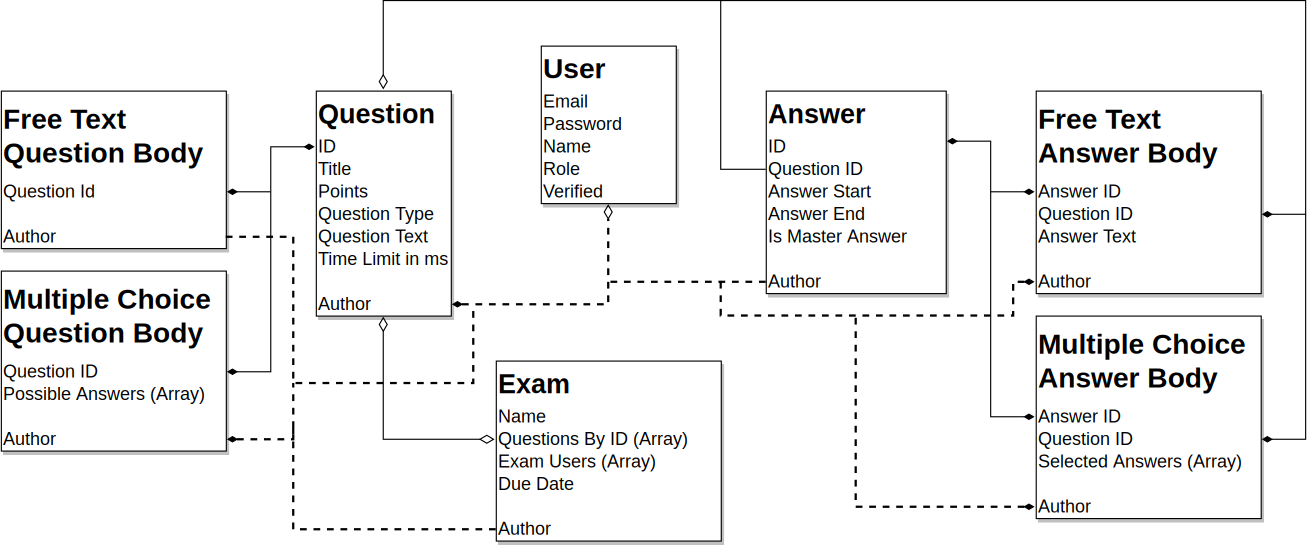
\includegraphics{../figures/dataModel.svg}
\caption{Data model of the prototype}
\end{figure}

One of the most important design considerations is the data model that
is used to store and access exam and user data. As is shown in figure 1,
there are four central instances: The most critical data instance is the
\emph{question}. Especially with the creation of question-pools in mind,
it is clear that these \emph{question instances} must live independently
of any exam. A question consists of a title, the question type, the
question text, the question's points, and the question's time limit.
Further, each question has a question body. The shape of the
question-body depends on the question type. For example, the
multiple-choice question-body consists of a reference to the question it
belongs to, and a selection of possible answers. For free-text
questions, no body is needed. Still, to be consistent in the data
structure, and to allow for later additions, free-text questions also
have a body.

These questions can then be assembled into the second central instance,
the exam. Each exam contains an exam name, the users that are allowed to
take part in a given exam, and an exam date. Most importantly, an exam
contains a list of question ids, which constitute the exam content.

The third central instance is the user. Users can either be examinees or
students with each having different permissions. Students, in contrast
to examiners, can not create exams or questions. If any new data
instance is created, e.g.~a new question, the \emph{author} property is
set to user performing the request. Further, users possess an email, a
password, a name, and a unique identifier property. The id is provided
by the application but could also be an identifier given by the testing
authority, as can be seen in figure \emph{2}. With user handling and
automatic assignment of authorship, we can ensure \emph{2.8} and, to a
large degree \emph{2.6} and \emph{2.7}.

The last key instance is the answer. For each question, an examinee
answers an \emph{answer instance} is created. This instance contains a
timestamp at which the question is started, a timestamp at which the
question was answered, and the question-id the answer is referring to.
Additionally, the answer object provides a flag that marks it as a
master answer. Master answers are the correct answers, or in the case of
free-text questions, provide a guideline of what is to be considered
correct. These master answers can only be created by examiners. Analog
to the question, the answer also bears an answer-body. The form of this
body again depends on the question type. \emph{Multiple-choice
answer-bodies} contain the selected answers, whereas \emph{free-text
answer-bodies} contain the given free-text answer. Additionally, any
answer body contains a reference to the answer and to the respective
question using its id.

\begin{figure}
\centering
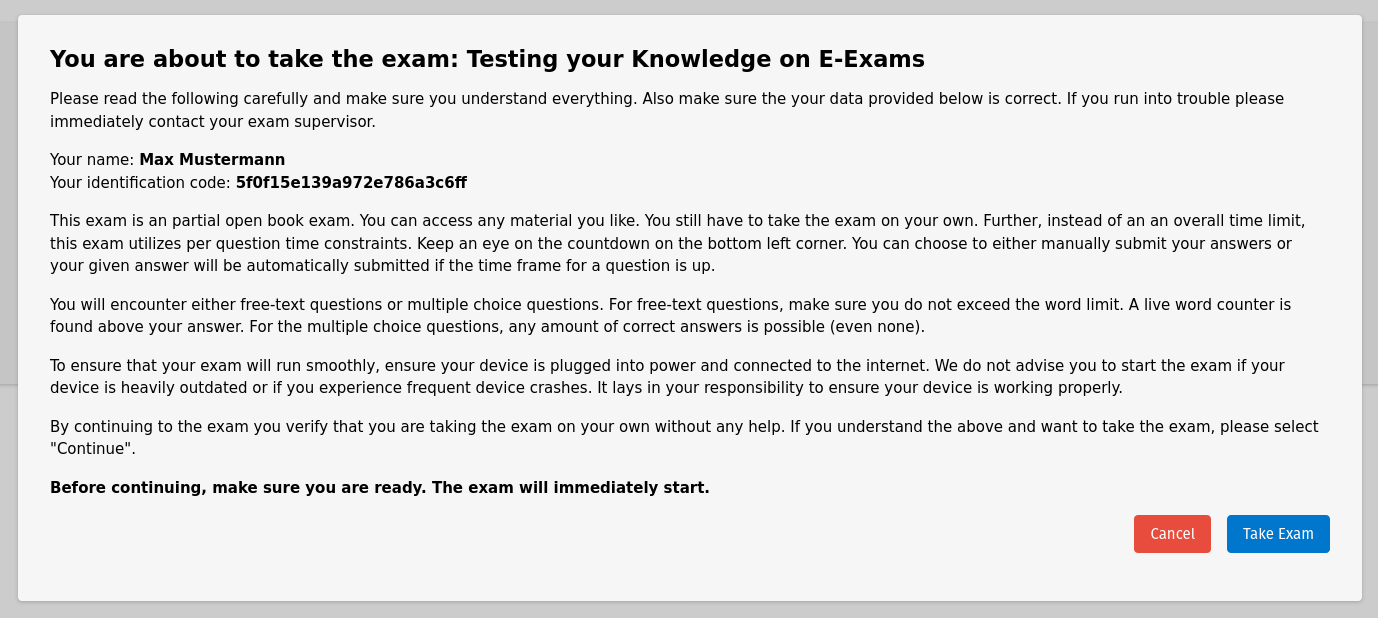
\includegraphics{../figures/startExamCrop.png}
\caption{Start screen of an exam with important user information,
e.g.~their name and user-id}
\end{figure}

The above provides an overview of the data structure, as it is found in
the database. As this app inhibits offline capabilities, large portions
of this data structure can again be found in the front-end application.
Of course, the data is reduced to the data that a user, e.g a student,
is allowed to see. Still, the structure of questions and answers remain
identical. To realize the mentioned offline capabilities, the exam data
persists in the local storage of the browser. Data remains in this local
storage until deleted by the app or intentionally removed by the user.
If there is an internet connection the data on the server and the data
in the local storage remain the same. Should the internet connection
fail, the exam continues as normal. Answers are then saved to the local
storage and at a later point in time, send to the server. Depending on
the circumstances students are taking their exams under, examiners can
adjust the degree of offline capabilities. Students could be allowed to
take their complete exam in offline mode. At the end of the exam are
they required to submit their answers. With the handling of offline
capabilities, we can ensure the requirement \emph{2.2}. Further,
critical information to ensure a save exam environment are provided at
the beginning of the exam. This can be seen in figure \emph{2}

\begin{figure}
\centering
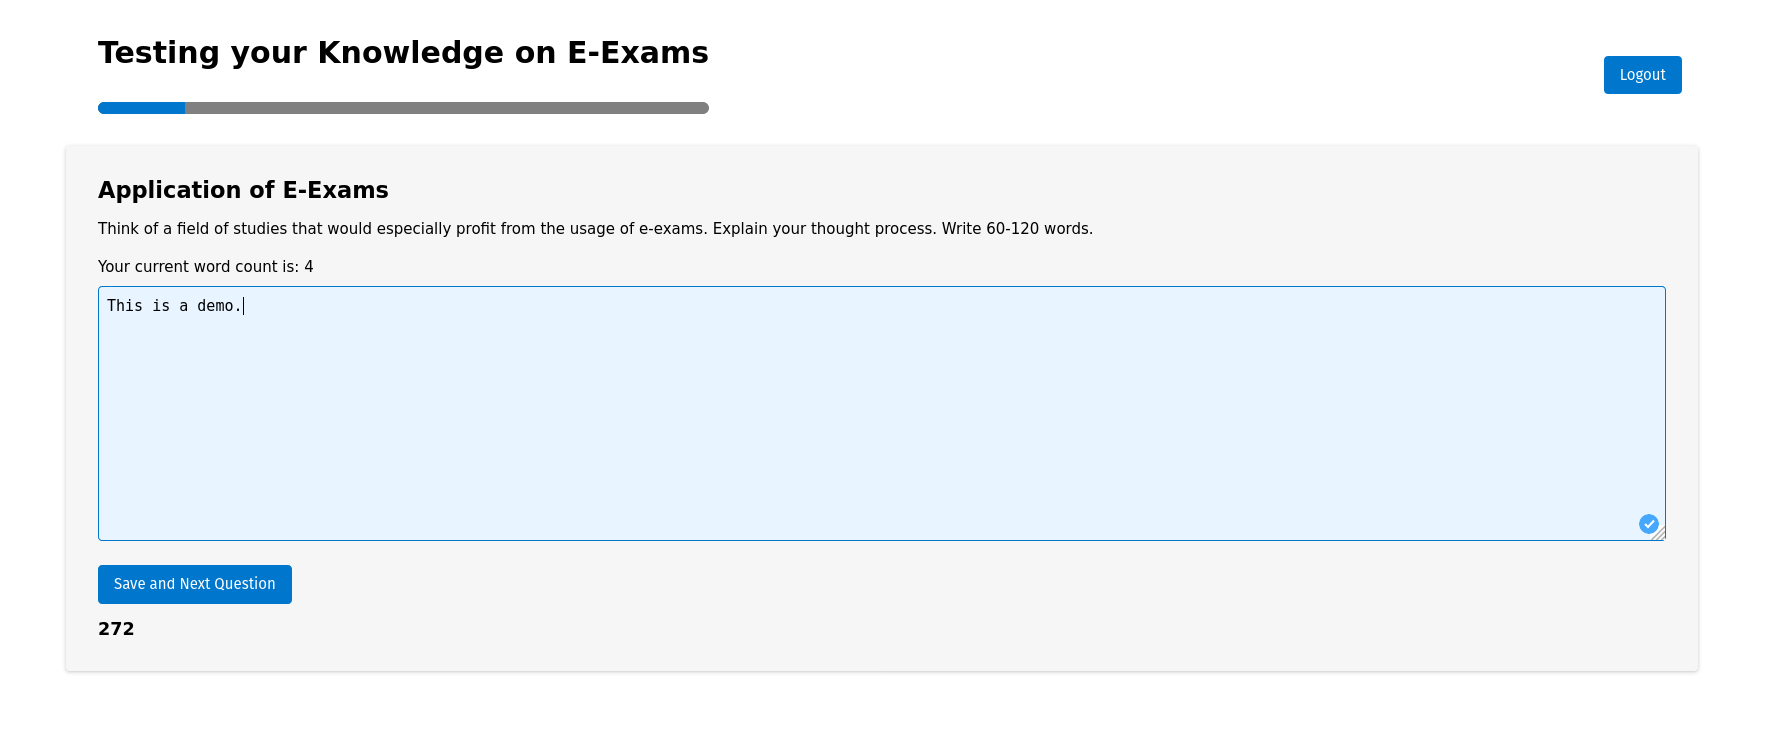
\includegraphics{../figures/answerCrop.png}
\caption{Answer field, with timer (bottom left)}
\end{figure}

To provide a way to meet requirement \emph{2.1.} and to fulfill parts of
the design principles to ensure \emph{2.4.}, the front-end application
must enforce per question time constraints. The back-end can review the
actual time used to give an answer. Still, the user interface must
assist the student in taking only as much time as allowed. The artifact
achieves this by showing the remaining time and submitting the currently
provided answer as soon as time is up, as seen in figure \emph{3}. This
answer is then sent to the server. Students are thus forced to comply
with the respective time constraints, leaving them no room to
accidentally miss allowed times, this can be seen in figure \emph{4}.

\begin{figure}
\centering
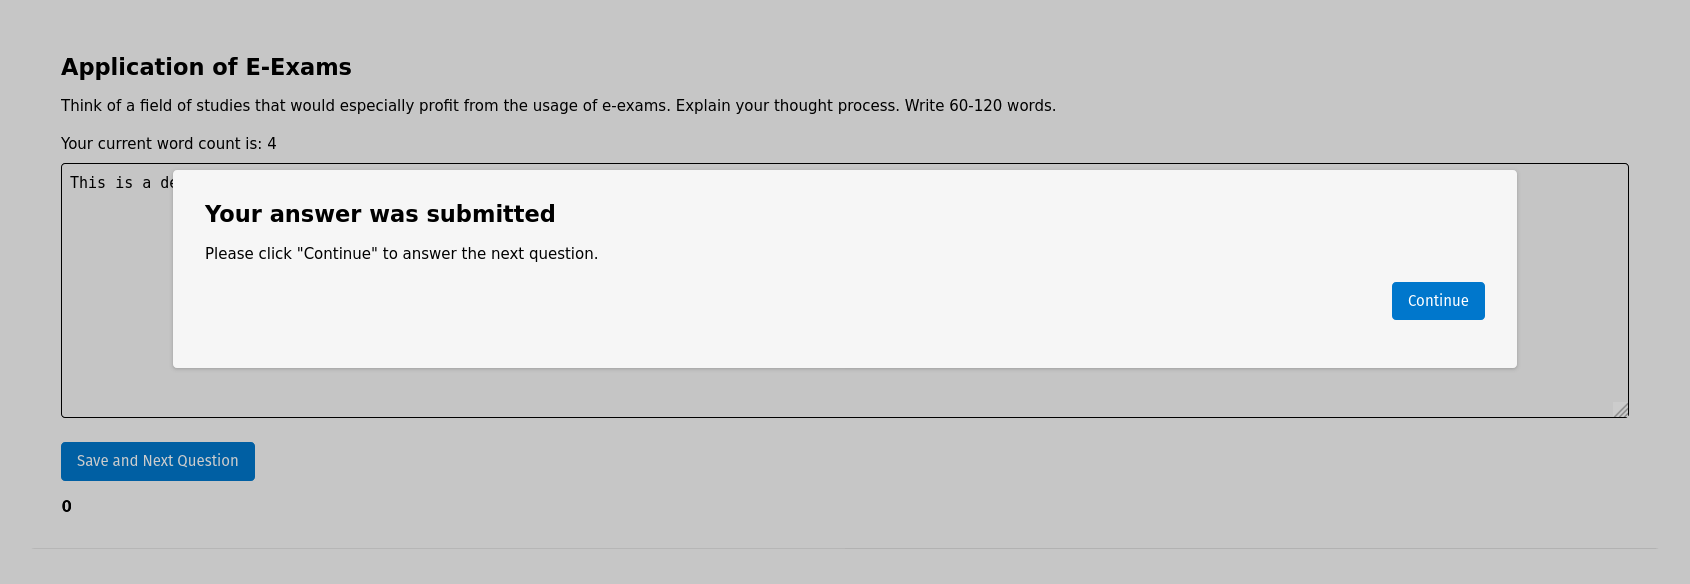
\includegraphics{../figures/nextQuestionCrop.png}
\caption{Automatic submission after time was depleted.}
\end{figure}

\newpage

\hypertarget{technologies-in-use}{%
\subsection{Technologies in Use}\label{technologies-in-use}}

Both the server and the client side are written in a coding language
called JavaScript. It is the most popular language on Github (Octoverse
\protect\hyperlink{ref-Octoverse}{2019}). JavaScript allows programmers
to realize a complete web app using only one language, making it a
compelling option when writing such an application. Besides, many modern
and popular libraries for web development are written in JavaScript.
Some libraries also find use in this artifact, the most crucial being
React created by Facebook and the Express framework (OpenJS Foundation
\protect\hyperlink{ref-Express}{2020}\protect\hyperlink{ref-Express}{a}).

React is ``a JavaScript library for building user interfaces'' (Facebook
Inc \protect\hyperlink{ref-FacebookInc}{2020}). It uses structures that
are divisible in reusable components. React makes it easy to create
complex applications instead of simple websites. It was originally
created by Facebook and finds its use in the tech-stacks of Uber,
Airbnb, Netflix and many more (Techstack
\protect\hyperlink{ref-Techstack}{2020}). Further the front-end uses the
JavaScript superset TypeScript. TypeScript allows to define and check
for complex types, whereas JavaScript in general is typless. These types
allow for more secure data handling, making the application overall less
prone to bugs. Lastly, an UI-library is used to create a visually more
pleasing experience.

Express is a common library for the creation of back-end services. It is
lightweight and allows for the creation of both simple and complex APIs.
As many back-end-applications rely on the same structure, generators for
the fundamentals exist. For this artifact, we used the \emph{Rest API
Generator} (Scholz and Gülcan \protect\hyperlink{ref-Scholz}{2020}). The
express server also handles data storage; for this purpose a database is
connected. The artifact uses a noSQL database called MongoDB.\footnote{https://www.mongodb.com/de/what-is-mongodb.}
MongoDB does not store data in tables, but in JSON-like documents. The
JSON format is inspired by JavaScript objects. Thus, the data structure
used in the front-end of the application, directly translates to the
data structure that is used to store the given data.

\hypertarget{future-implementations}{%
\subsection{Future Implementations}\label{future-implementations}}

As the artifact is only a proof of concept and no market-ready software,
it lacks some key features. Exams, for example, can be conducted, but
there is no way of evaluating them through a user interface. As the
correction of exams is not implemented yet, the \emph{2.5} remains
unmatched.

Further, the video and sound surveillance are not implemented yet. Thus,
Protection against cheating remains also partially unmatched. As can be
seen above, the video supervision only addresses the aspect of cheating
by the use of outside help. Looking at table 1, this supervision of
students is the only measure against cheating that is not enforced.

We have looked at large question pools in section \emph{2.} In theory,
in the current software artifact, there is a way of creating such
question pools. However, there are some limitations: For the creation of
large question pools, crowd collaboration can be used. Universities have
created questions for numerous years. As these questions leak or get
published, these become worthless for a single institution. Sharing
them, opens questions up to new uses. To enable the common sharing of
questions two things must be achieved. First. a common question format
must be found. The data structure of the question-type of this artifact
could theoretically serve such a purpose. Second, a platform is needed
to share questions. Such a platform should also take care of some kind
of quality assurance. At the time of writing, such a platform does not
exist.

Lastly, this artifact serves as a minimal viable product, many of the
user interactions are not suited for large amounts of data. Regarding
the further development of the app, usability and performance must
continuously be evaluated and improved.

\newpage

\hypertarget{conclusion}{%
\section{Conclusion}\label{conclusion}}

First, this thesis argued that the advantages of e-exams can only be
leveraged, if all requirements for a sound assessment tool are met. We
gave intuition, which design principles allow us to create such an
e-exam. As a major aspect of e-exams we put forth the idea of partial
open-book exams, making use of per question time constraints. Besides,
we stressed the importance of offline capabilities as a way of
protection against contestation and assessed how e-exams can enforce
time constraints to counteract cheating.

Further, we evaluated these design principles on a multitude of software
products. None of these products achieved to meet all the requirements.
Some of the major shortcomings included the lack of the above-mentioned
time restrictions, missing offline capabilities and the missing of
continuos identity evaluation. The lack of a suitable examination tool
has motivated the development process of a software artifact that
implements all the discussed design principles. This thesis provides a
prototype of such a software artifact. It enforces time restrictions and
has offline capabilities, in that way addressing the main shortcomings
of the other, market ready software solutions.

As an outlook, the development of an e-examination tool is only part of
the whole assessment process. The creation of the actual questions is a
second important and time-consuming aspect. As already mentioned above,
e-exams rely on large question pools. At the moment, no feasible way of
sharing questions on a large scale exists. Such a sharing
infrastructure--whether integrated into the exam tool or
standalone--could largely improve the assessment process. Through
collaborative effort such a platform could also improve the overall
quality of questions asked in exams.

To conclude, this thesis has proposed design principles that can be used
to create a valid e-examination software. Further, it provides a
software artifact that embeds key design principles. Although, this
prototype is by no means market-ready it provides a starting point for a
software that allows for valid and decentralized e-exams.

\newpage

\hypertarget{declaration}{%
\section{Declaration}\label{declaration}}

Ich versichere hiermit wahrheitsgemäß, die Arbeit selbstständig verfasst
und keine anderen als die angegebenen Quellen und Hilfsmittel benutzt,
die wörtlich oder inhaltlich übernommenen Stellen als solche kenntlich
gemacht und die Satzung des Karlsruher Instituts für Technologie (KIT)
zur Sicherung guter wissenschaftlicher Praxis in der jeweils gültigen
Fassung beachtet zu haben.

Karlsruhe, den 23.09.2020: \hrulefill\newline
\phantom{Karlsruhe, den 23.09.2020: }Jasper Anders

\newpage

\hypertarget{references}{%
\section{References}\label{references}}

\hypertarget{refs}{}
\begin{cslreferences}
\leavevmode\hypertarget{ref-XM-Backend}{}%
Anders, Jasper. 2020a. ``Github Page of the XM Prototype Backend.''
\url{https://github.com/jasperanders/XM-Api}.

\leavevmode\hypertarget{ref-XM-Frontend}{}%
---------. 2020b. ``Github Page of the XM Prototype Frontend.''
\url{https://github.com/jasperanders/XM}.

\leavevmode\hypertarget{ref-Cluskey2011}{}%
Cluskey, G R, Craig R Ehlen, and Mitchell H Raiborn. 2011. ``Thwarting
online exam cheating without proctor supervision.'' \emph{Journal of
Academic and Business Ethics} 4: 1--8.
\url{http://search.proquest.com/docview/876280909/fulltextPDF?accountid=4840}.

\leavevmode\hypertarget{ref-ETSTOEFL}{}%
ETS TOEFL. 2020. ``Proctoring at Toefl.''
\url{https://www.ets.org/s/cv/toefl/at-home/test-day/}.

\leavevmode\hypertarget{ref-FacebookInc}{}%
Facebook Inc. 2020. ``React.'' \url{https://reactjs.org/}.

\leavevmode\hypertarget{ref-Gehringer2004}{}%
Gehringer, Edward F. 2004. ``Reuse of Homework and Test Questions :
When, Why, and How to Maintain Security ?''

\leavevmode\hypertarget{ref-Halbherr2014}{}%
Halbherr, Tobias, Kai Reuter, Daniel Schneider, Claudia Schlienger, and
Thomas Piendl. 2014. ``Making Examinations more Valid, Meaningful and
Motivating: The Online Exams Service at ETH Zurich.'' \emph{Eunis
Journal of Higher Education IT}, no. 1: 14.
\url{https://doi.org/10.13140/2.1.4635.1044}.

\leavevmode\hypertarget{ref-Handke2012}{}%
Handke, Jürgen, and Anna Maria Schäfer. 2012. \emph{E-Learning,
E-Teaching und E-Assesment in der Hochschullehre: Eine Anleitung}.
Oldenbourg Verlag München.

\leavevmode\hypertarget{ref-Hevner2004}{}%
Hevner, Alan R, Salvatore T March, Jinsoo Park, Sudha Ram, and Sudha
Ram. 2004. ``Research Essay Design Science in Information.'' \emph{MIS
Quarterly} 28 (1): 75--105. \url{https://doi.org/10.2307/25148625}.

\leavevmode\hypertarget{ref-James1927}{}%
James, H. W. 1927. ``The Effect of Handwriting upon Grading Published by
: National Council of Teachers of English Stable URL :
http://www.jstor.org/stable/803599.'' \emph{The English Journal} 16 (3):
180--85.

\leavevmode\hypertarget{ref-JohannesGutenberg-UniversitatMainz}{}%
Johannes Gutenberg-Universität Mainz. 2018. ``E-Klausuren an der Uni
Mainz.'' \url{https://www.elearning.uni-mainz.de/e-klausuren/}.

\leavevmode\hypertarget{ref-Mccabe2005}{}%
McCabe, Donald L. 2005. ``Cheating among college and university
students: A North American perspective.'' \emph{International Journal
for Educational Integrity} 1 (1).
\url{https://doi.org/10.21913/ijei.v1i1.14}.

\leavevmode\hypertarget{ref-Octoverse}{}%
Octoverse. 2019. ``Githubs top languages.''
\url{https://octoverse.github.com/\#top-languages}.

\leavevmode\hypertarget{ref-Express}{}%
OpenJS Foundation. 2020a. ``Express.js.'' \url{https://expressjs.com}.

\leavevmode\hypertarget{ref-Node}{}%
---------. 2020b. ``Node.js.'' \url{https://nodejs.org/}.

\leavevmode\hypertarget{ref-GLM2015}{}%
Peregoodoff, Robert. 2015. ``E-Examinations: Chances and Challenges.''
GML² 2015.

\leavevmode\hypertarget{ref-Scholz}{}%
Scholz, Jonas, and Tayfun Gülcan. 2020. ``Express API Generator.''
\url{https://github.com/tguelcan/restexpress}.

\leavevmode\hypertarget{ref-Techstack}{}%
Techstack. 2020. ``Who uses React?'' \url{https://stackshare.io/react}.

\leavevmode\hypertarget{ref-Vogt2009}{}%
Vogt, Michael, and Stephan Schneider. 2009. ``E-Klausuren an
Hochschulen.'' \emph{Koordinationsstelle Multimedia
Hochschulrechenzentrum Justus-Liebig-Universität Gießen}.

\leavevmode\hypertarget{ref-WELSH2004}{}%
Welsh, Brandon C., and David P. Farrington. 2004. ``Surveillance for
Crime Prevention in Public Space: Results and Policy Choices in Britain
and America'' 3 (3): 497--526.
\url{https://doi.org/10.1111/j.1745-9133.2004.tb00058.x}.
\end{cslreferences}
